
\medskip

\parbox{0.15\linewidth}{
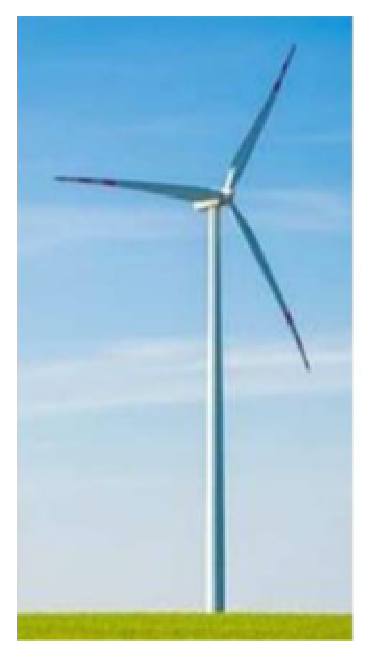
\includegraphics[width=2cm]{eolienne}}
\hfill
\parbox{0.55\linewidth}{On cherche à dessiner une éolienne avec le logiciel Scratch ; elle est formée de $3$ pales qui tournent autour d'un axe central.}\hfill 
\parbox{0.20\linewidth}
{
\psset{unit=0.01cm}
\def\pale{\pspolygon(0,0)(30,0)(30,13)(179.43,0)(30,-13)(30,0)}%ABEDCBA
\psset{linecolor=blue,unit=0.01cm}
\begin{pspicture}(-100,-6)(100,100)
\multido{\n=90+120}{3}{\rput{\n}(0,0){\pale}}
\rput(0,-105){Éolienne modélisée par Scratch}
\end{pspicture}
}
\medskip


\begin{tabularx}{\linewidth}{X m{3.5cm}}
\textbf{1.} La figure ci-dessous représente une pale d'éolienne.

\psset{unit=0.05cm}
\begin{pspicture}(-5,-25)(180,25)
%\psgrid
\pspolygon(0,0)(30,0)(30,13)(179.43,0)(30,-13)(30,0)%ABEDCBA
\psframe(30,0)(26,4)
\uput[u](0,0){A} \uput[r](30,0){B} \uput[u](30,13){E} \uput[r](179.43,0){D} \uput[d](30,-13){C} \uput[u](15,0){30}\uput[u](105,6.5){150}\uput[l](30,-6.5){13}
\rput(30,6.5){$\bullet$}\rput(30,-6.5){$\bullet$}
\psline(107,9)(105,5)\psline(105,-9)(107,-5)
\psarc(30,-13){5}{10}{90}\rput(40,-8){\footnotesize $85\degres$}
\end{pspicture}

-- DEC est un triangle isocèle en D;

-- B est le milieu de [EC] ;

-- [AB] est perpendiculaire à [EC] ; 

-- $\widehat{\text{ECD}}= 85\degres$.

\qquad \textbf{a.~} Montrer que l'angle $\widehat{\text{CDE}} = 10\degres$.

\qquad \textbf{b.~} Le script \og pale \fg{} ci-contre permet de tracer une pale de l'éolienne avec le logiciel Scratch.

Pourquoi la valeur indiquée dans le bloc de la ligne \no 6 est-elle 95 ?

\qquad \textbf{c.~} Dans ce même script \og pale \fg{}, par quelle valeur doit-on compléter le bloc situé à la ligne \no 8 ? 

Recopier cette valeur sur votre copie.

\textbf{2.~} Le script \og éolienne \fg{} ci-contre permet de tracer l'éolienne avec le logiciel Scratch.

Par quelle valeur doit-on compléter la boucle \og  répéter\fg{} ? Recopier cette valeur sur votre copie.
&~
\setscratch{scale=.75}
\begin{scratch}[num blocks]
\initmoreblocks{définir \namemoreblocks{pale}}
\blockpen{stylo en position écriture}
\blockmove{avancer de \ovalnum{30}}
\blockmove{tourner \turnright{} de \ovalnum{90} degrés}
\blockmove{avancer de \ovalnum{13}}
\blockmove{tourner \turnleft{} de \ovalnum{95} degrés}
\blockmove{avancer de \ovalnum{150}}
\blockmove{tourner \turnleft{} de \ovalnum{} degrés}
\blockmove{avancer de \ovalnum{150}}
\blockmove{tourner \turnleft{} de \ovalnum{95} degrés}
\blockmove{avancer de \ovalnum{13}}
\blockmove{tourner \turnright{} de \ovalnum{90} degrés}
\blockmove{avancer de \ovalnum{30}}
\blockmove{tourner \turnright{} de \ovalnum{180} degrés}
\blockpen{relever le stylo}
\end{scratch}

\begin{scratch}
\initmoreblocks{définir \namemoreblocks{éolienne}}
\blockmove{aller à x: \ovalnum0 y: \ovalnum0}
\blockrepeat{répéter \ovalnum{} fois}
{\blockmoreblocks{pale}
\blockmove{tourner \turnright{} de \ovalnum{120} degrés}
}
\end{scratch}\\
\end{tabularx}



